\htwo{Webspeicher}
\label{sec:webstorage}
\sectionauthor{Johannes Polzer}

\hthree{Einleitung}

Webspeicher (im Englischen "Web Storage" genannt) ermöglichen den Entwicklern % tofix: Gendern? 
Daten im Webbrowser zu speichern.
Es gibt verschiedene Arten von Webspeichern, welche für unterschiedlicher Anwendungsfälle konzipiert wurden. Dazu zählen:

\begin{itemize}
    \item Local Storage
    \item Session Storage
    \item Cookies
    \item Indexed-DB
    \item Cache
\end{itemize}

Damit die Daten nicht von anderen Web-Apps gelesen und manipuliert werden können, kommt eine  "Same-Origin-Policy" zum Einsatz (siehe Kapitel \ref{sec:sameorigin}).
% Damit die Session gespeichert und die Website offline aufgerufen werden kann, ist es wichtig, Daten im Webbrowser abzuspeichern. Es gibt verschiedene Arten von Speichern in einem modernen Webbrowser Um riesige Webanwendungen zu entwickeln, wurde die Menge an Speicherplatz in den letzten Jahren erhöht. 

\hfour{Speichermengen}

Damit eine Webanwendung nicht die gesamte Festplatte vollschreiben kann, wird die Speichermenge einer Webseite limitiert. Diese Limitierungen sind davon abhängig, welcher Webbrowser verwendet wird.

Der Google Chrome Browser erlaubt es, Webseiten bis zu achtzig Prozent der Fest\-platten\-kapazität zu nutzen.

Firefox hat ein Limit von zwei Gigabyte pro Website. Insgesamt dürfen Webseiten bis zu 50 \% des freien Speicherplatzes nutzen.

Apples Safari-Browser schränkt die Nutzung von Webanwendungen auf maximal ein Gigabyte ein. Wenn diese Grenze erreicht ist, wird der Benutzer alle 200 MB gefragt, ob er weitere 200 MB zulassen möchte. Dieses Verhalten ist jedoch von Apple nicht dokumentiert. \cite{WebDevStorage}

\hfour{Same-Origin-Policy} \label{sec:sameorigin}

Damit nicht jede Webseite auf die gespeicherten Ressourcen der anderen Webseiten zugreifen kann, gibt es eine "Same-Origin-Policy".
Dadurch soll verhindert werden, dass Webseiten andere Webseiten ausspionieren, indem sie auslesen, mit welchen Accounts der Benutzer auf anderen Seiten angemeldet ist. Außerdem wird die Manipulation der Daten anderer Seiten unterbunden. \cite{MDNSame-origin-policy}

Dennoch kann Tracking mit Hilfe von Cookies durchgeführt werden.
Dabei wird auf einer Webseite \zb\ ein Script von Google Analytics eingebunden. Dieses Script kann dann auf die Daten der anderen Webseiten zugreifen und somit mit Tracking-Cookies das Benutzer\-verhalten verfolgen.


\hthree{Allgemeines}

\hfour{Local Storage}\label{sec:localstorage}

Im Local Storage können Strings gespeichert werden. Dieser Speicher wird nie gelöscht, es sei denn, die Benutzer tun es selbst. 
\cite{w3LocalStorage}

\typescript{code/Webspeicher/localstorage.ts}{Schreiben und Lesen des Local-Storage}
\hfour{Session Storage}

Der Session Storage ist dem Local Storage (Kapitel \ref{sec:localstorage}) sehr ähnlich. 
Der einzige Unterschied ist, dass die Daten nach dem Schließen der Sitzung bzw. beim Beenden der Webapp gelöscht werden.

\typescript{code/Webspeicher/sessionstorage.ts}{Schreiben und Lesen des Session-Storage}

\hfour{Cookies}

Web-Cookies sind Dateien auf einem Client-Gerät, die von einem Webserver übermittelt werden, um Clients zu identifizieren. 
Bei der ersten Anfrage sendet ein Server die Webseite selbst und zusätzlich ein Cookie zurück. 
Dieses Cookie wird bei jeder weiteren Anfrage automatisch an den Server gesendet und kann dort aktualisiert werden. 
Da Cookies nach Beenden der Sitzung nicht gelöscht werden, werden diese auch bei erneuten Aufrufen mitgeschickt, wodurch \zb\ ermöglicht wird, dass der Benutzer auf einer Webapp angemeldet bleibt. 

Allerdings ist es auch möglich, Cookies mit Javascript zu speichern. %, welches vom Server mit der Webseite mitgesendet wird. 
\cite{wikiCookies}

\hfour{Indexed-DB}\label{sec:indexeddb}

Eine neue Entwicklung zur Speicherung von großen Datenmengen ist die Indexed-DB. 
Diese ist eine Datenbank, welche den Entwicklern ermöglicht, Daten in der Form von Objekten abzuspeichern.

Jede Datenbank enthält sogenannte Object-Stores. Das sind Sammlungen von Daten, welche als JSON-Objekte abgespeichert sind. 
Im Gegensatz zu relationalen Datenbanken ist bei der Indexed-DB kein festes Schema erforderlich. 
Dennoch ist immer ein Primärschlüssel zu definieren, welcher in diesem Object-Store für jedes Objekt einzigartig sein muss.
Dieser kann entweder ein Attribut des Objektes sein oder durch eine automatisch inkrementierende Ganzzahl generiert werden. 

Damit Datensätze nach einer Eigenschaft durchsucht werden können, wird ein Index erstellt. 
Ein indiziertes Attribut muss in jedem Objekt des Object-Stores vorhanden sein.

Im Vergleich zu Session-Storage und Local-Storage ist die API der Indexed-DB komplexer zu implementieren.

Um mit Indexed-DB arbeiten zu können, wird zunächst ein sogenannter "open request" erstellt:

\typescript{code/Webspeicher/openRequest.ts}{Erstellen eines Indexed-DB Open-Requests}

\begin{figure}[H]
    \centering
    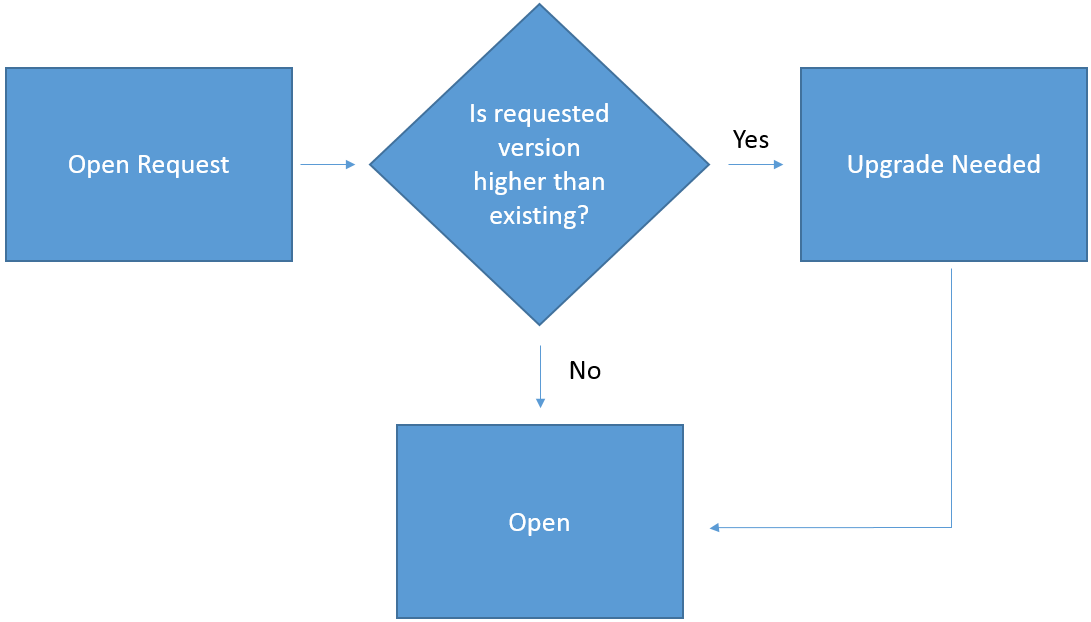
\includegraphics[width=0.8\textwidth]{media/Webspeicher/openDb.png}
    \caption{Öffnen einer Indexed-DB \cite{fig:openDB}}
\end{figure}

Auf dem Open-Request-Objekt gibt es mehrere Events. 
Das Event "{\ttfamily upgradeneeded}" wird ausgelöst, wenn die geöffnete Datenbank noch nicht initialisiert wurde oder wenn die Version erhöht wurde. 
Die Version der Datenbank wird beim Erstellen des Open-Requests angegeben. 
Wenn sich das Schema der Datenbank ändern soll, wird diese Versionsnummer erhöht, damit das "{\ttfamily upgradeneeded}"-Event ausgelöst wird.
Innerhalb dieses Ereignisses werden die Object-Stores und die Indizes erstellt (siehe Code \ref{code:createDB}). 
Beim Erstellen des Object-Stores müssen der Name des Object-Stores und der Primärschlüssel definiert werden. Wenn der Primärschlüssel automatisch generiert werden soll, muss dies durch die Eigenschaft "autoIncrement", welche auf "true" gesetzt werden muss, angegeben werden.
Wenn der Object-Store erstellt ist, können Attribute indiziert werden. 
Dabei muss jedem Index ein Name gegeben und ein Attribut angegeben werden, nach welchem der Object-Store durchsucht werden soll. 
Außerdem kann definiert werden, ob dieses Attribut einzigartig (unique) sein soll.

\typescript[code:createDB]{code/Webspeicher/createDB.ts}{Erstellen und Ändern des Datenbankschemas}

Das Event "{\ttfamily success}" wird nach der vollständigen Initialisierung der Datenbank ausgelöst -- 
das heißt, nach dem "{\ttfamily upgradeneeded}"-Event, falls dieses erforderlich war. 
Wenn die Datenbank bereits initialisiert wurde, wird das "{\ttfamily success}"-Event sofort ausgelöst. 
Nach dem "{\ttfamily success}"-Event sind alle Arten von Manipulationen und Abfragen der Daten möglich. 
Zum Abrufen von Daten aus der Indexed-DB, wird eine Transaktion unter Verwendung des "Indexed Database Objekts" erstellt. 
Das "Indexed Database Objekt" ist als Ergebnis des "Open Request" abrufbar.

\typescript{code/Webspeicher/getByPrimaryKey.ts}{Abfragen von Datensätzen mit einem Primärschlüssel}

Es ist auch möglich, Daten über einen Index abzurufen. Da ein indiziertes 
% Zusammenhang methoden First/all Match
Attribut nicht eindeutig sein muss, gibt es zwei Methoden, um die Daten zu erhalten. Die Methode "{\ttfamily get}" liefert die erste Übereinstimmung und die Methode "{\ttfamily getAll}" alle Über\-ein\-stimmungen als Array.

\typescript{code/Webspeicher/getByIndex.ts}{Abfragen von Datensätzen mit einem Index}

Die Add-Methode des Object Stores erlaubt es Objekte hinzuzufügen. Die Put-Methode überschreibt bestehende Objekte.
\cite{MDNIndexedDB}
\cite{MDNUsingIndexedDB}
\clearpage
\hfour{Cache API}

Die Cache-API ermöglicht das Zwischenspeichern von Websites für eine Offline-Nutzung. Sie werden meist in PWAs verwendet. Der Code für die Zwischenspeicherung wird in einem Service Worker geschrieben, der ein JavaScript ist, das auf einem separaten Thread läuft. Die Verwendung der Cache-API wird im Beispiel vom Service Worker Kapitel \ref{sec:cacheImpl} gezeigt.
\clearpage

\hfour{Speicherung des JWT}

Um den JSON Web Token sicher zu speichern, ist es wichtig, dass dieser nicht mit unbegrenzter Gültigkeit gespeichert wird. Darüber hinaus soll der Administrator beim Schließen des "Admin Dashboards" ausgeloggt werden. Deshalb wird dieser Token im Session-Storage abgelegt. Dadurch wird der Token nach der Sitzung gelöscht und der Administrator muss sich beim nächsten Besuch des "Admin Dashboards" neu anmelden.

\hfour{Cache für schnelle Ladezeiten}

Damit die Anwendung alle Voraussetzungen erfüllt um als PWA installiert zu werden, muss die Webseite im Cache gespeichert werden. Somit kann die Webseite bzw. die installierte PWA offline genauso geöffnet werden. Allerdings wird bei der offline-Nutzung eine Meldung angezeigt, dass keine Rauminformationen verfügbar sind, da die API-Anfragen eine Aktive Internetverbindung benötigen.

Ein Beispiel für die Implementierung des Cache (Code \ref{code:cache}) befindet sich im Kapitel \ref{sec:cacheImpl} auf Seite \pageref{code:cache}.
 